\section{Superheterodynmottagare}
\textbf{
HAREC a.\ref{HAREC.a.4.1.1a}\label{myHAREC.a.4.1.1a},
 a.\ref{HAREC.a.4.3.1}\label{myHAREC.a.4.3.1},
 a.\ref{HAREC.a.4.3.4}\label{myHAREC.a.4.3.4}
}
\index{superheterodynmottagare}
\index{mottagare!superheterodyn}
\index{super}
\index{mottagare!super}

Superheterodynprincipen ger mycket större möjligheter, när önskemålet
är en högselektiv mottagare för flera olika frekvenser.

Skillnaden mellan en direktblandad mottagare och en
\emph{superheterodynmottagare}, ofta bara kallad ''super'' eller
''superhetero'', är att blandningsprodukterna i direktblandaren blir till
LF direkt, medan de i supern först bildar en mellanfrekvenssignal MF,
vilken sedan demoduleras och LF-detekteras.

I det följande kallas superheterodynmottagaren enbart \emph{super}.
I supern blandas de mottagna signalerna med signalen från en VFO.
Före blandningen har HF-signalerna passerat ett selektivt försteg, som
dämpar spegelfrekvenser.
För att inte störa mottagningen placeras VFO-frekvensen alltid utanför
det frekvensband, där man vill ta emot signaler.

Alla mottagna signaler blandas med VFO-signalen.
Mottagningsfrekvensen är vanligen skillnaden mellan en fast så kallad
mellanfrekvens MF och VFO-frekvensen.
Mellanfrekvensen är egentligen mittfrekvensen i ett fast passband skapat av
ett antal filter.

\begin{figure}
  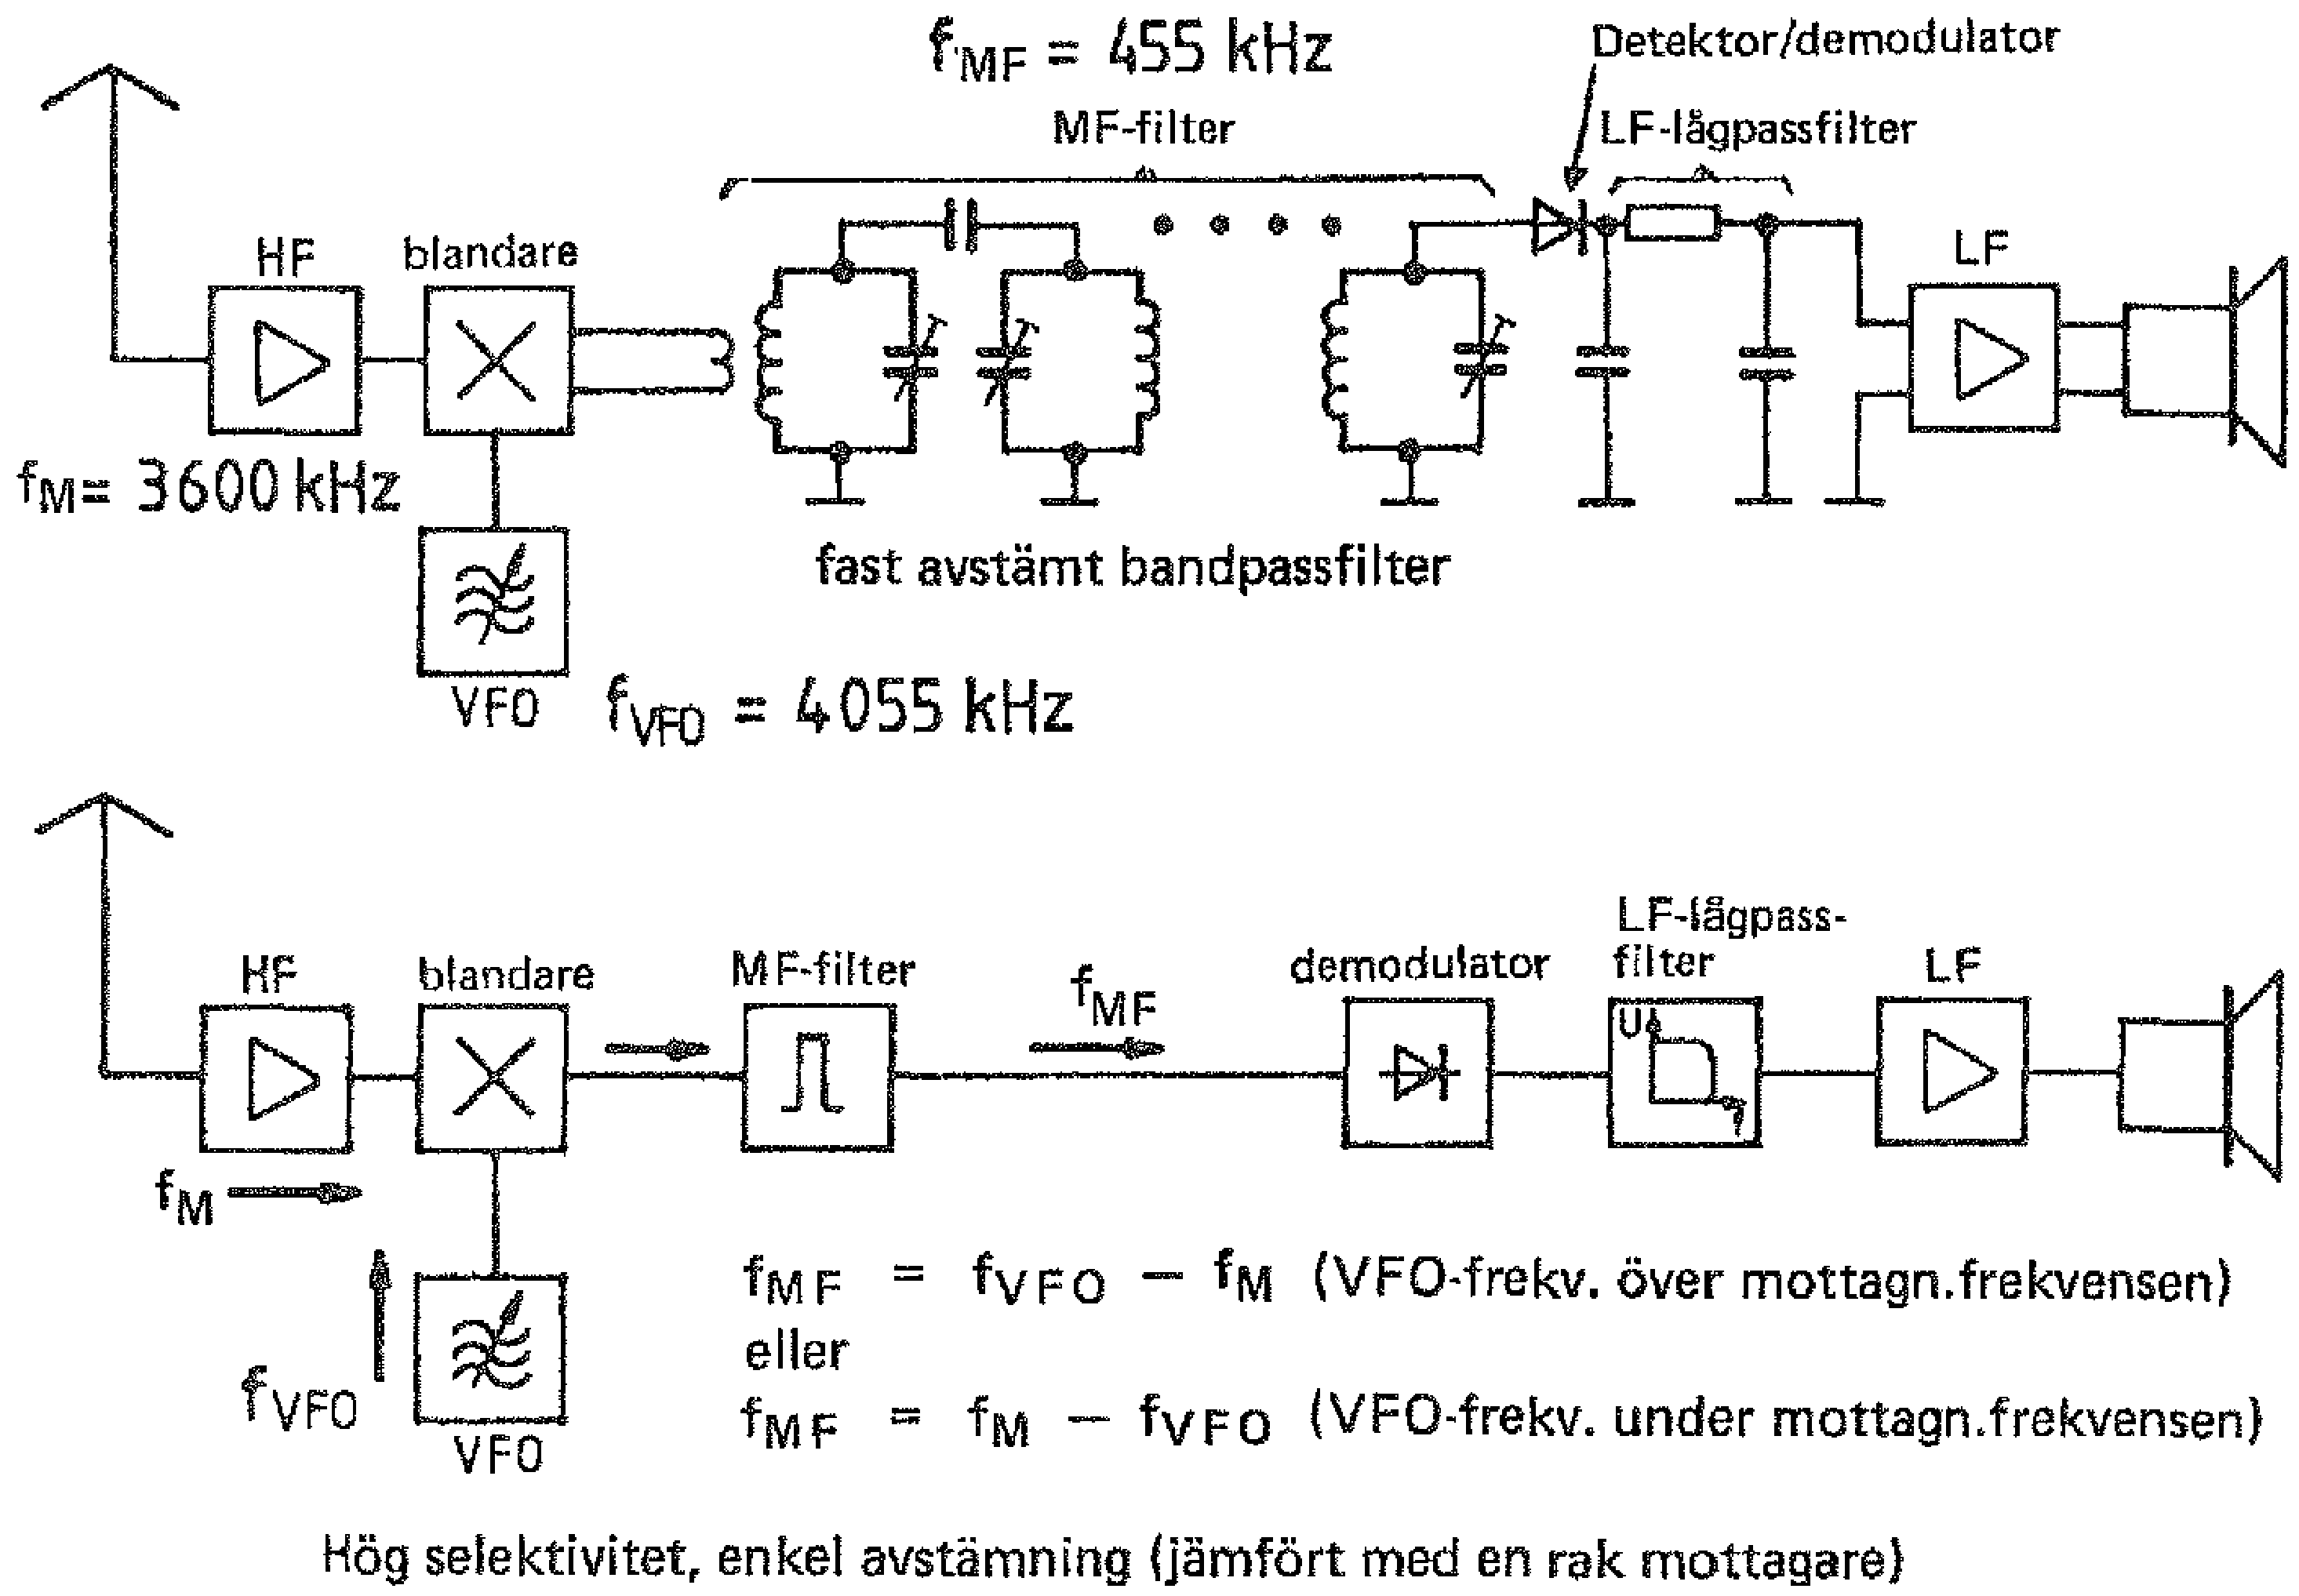
\includegraphics[width=\textwidth]{images/cropped_pdfs/bild_2_4-13.pdf}
  \caption{Superheterodynmottagaren i princip}
  \label{fig:bildII4-13}
\end{figure}

Bild \ref{fig:bildII4-13} visar en mottagare med mellanfrekvensen 455~kHz,
som är vanlig i äldre mottagare.
MF-filtret kan i enklaste fall bestå av ömsesidigt magnetiskt kopplade
LC-svängningskretsar.
Bättre avstämningsskärpa fås med resonatorer av keramik eller kvarts eller med
hjälp av elektromekaniska resonatorer.

\textbf{Exempel:}
En sändning på frekvensen 3600~kHz ska tas emot.
Vi ställer då in VFO-frekvensen till 4055~kHz, eftersom mellanfrekvensen är
\(4055 - 3600 = 455\)~kHz.
Den mottagna signalen hamnar då mitt i MF-filtrets passband.

Signaler på angränsande frekvenser tas också emot och alstrar
blandningsprodukter.
Med ett mellanfrekvensfilter med till exempel 3~kHz bandbredd (453,5--456,5~kHz),
kan signalfrekvenser mellan 3598,5 och 3601,5~kHz passera genom filtret.
En signal med en närliggande frekvens till exempel 3603~kHz, och blandad med den
inställda VFO-frekvensen 4055~kHz, kommer att alstra en skillnadsfrekvens av
452~kHz.
Denna signal ligger utanför filtrets passband och kommer att dämpas och når
inte detektorn.

VFO-signalen kan givetvis läggas under i stället för över mellanfrekvensen.

\textbf{Exempel:}
VFO-frekvensen 3145~kHz kan också användas för mottagning av frekvensen
3600~kHz, om mellanfrekvensen är 455~kHz (\(3600 - 455 = 3145\)~kHz).
Men för att undvika att eventuella övertoner från VFO-signalen blandas med
mottagna signaler är det lämpligt att placera VFO-frekvensen över
mottagningsfrekvensen.

Efter MF-filtren följer bland annat detektorer för olika sändningsslag samt
LF-förstärkare.
Jämför med bild \ref{fig:bildII4-5} och \ref{fig:bildII4-6}.

\subsection{Dubbelsuperheterodynmottagare}
\textbf{HAREC a.\ref{HAREC.a.4.1.1b}\label{myHAREC.a.4.1.1b}}
\index{dubbelsuperheterodynmottagare}
\index{mottagare!dubbelsuperheterodyn}

Det är svårt att bygga enkla mellanfrekvensfilter för höga frekvenser,
med liten bandbredd och branta flanker. Det är fallet för en
enkelsuper för kortvåg med en enda mellanfrekvens, till exempel 9~MHz.

En god närselektion på höga frekvenser är endast möjlig med relativt
dyrbara kristallfilter.
Däremot går det att få god närselektion med enklare medel på lägre frekvenser.

En dubbelsuper, det vill säga en super med dubbel frekvensomvandling,
möjliggör god både när- och förselektion, illustreras i bild
\ref{fig:bildII4-14}.
I 1:a blandaren blandas den mottagna signalen med signalen från en
1:a oscillator (VFO) till en hög mellanfrekvens, till exempel 9 eller 10,7~MHz.

Därmed kan en god spegelfrekvensdämpning erhållas.
Första MF-filtret kan göras enklare och utan den höga selektivitet som hade
behövts i en enkelsuper.
1:a MF blir sedan blandad ytterligare en gång i 2:a blandaren till en 2:a MF,
till exempel 455~kHz.
För den andra blandningen används en fast oscillator.
Filtret i 2:a MF kan lättare utföras med en hög selektivitet, på grund av den
lägre frekvensen.

\textbf{Exempel:}
Trots att MF-filtret inte är en enkel svängningskrets, kan ett ''Q-värde''
beräknas.
Vid en passbandbredd av 6~kHz och en centerfrekvens av 455~kHz kan Q-värdet
anses vara

\[ Q = \frac{f_{res}}{b} = \frac{455}{6} = 76 \]

\begin{figure}
  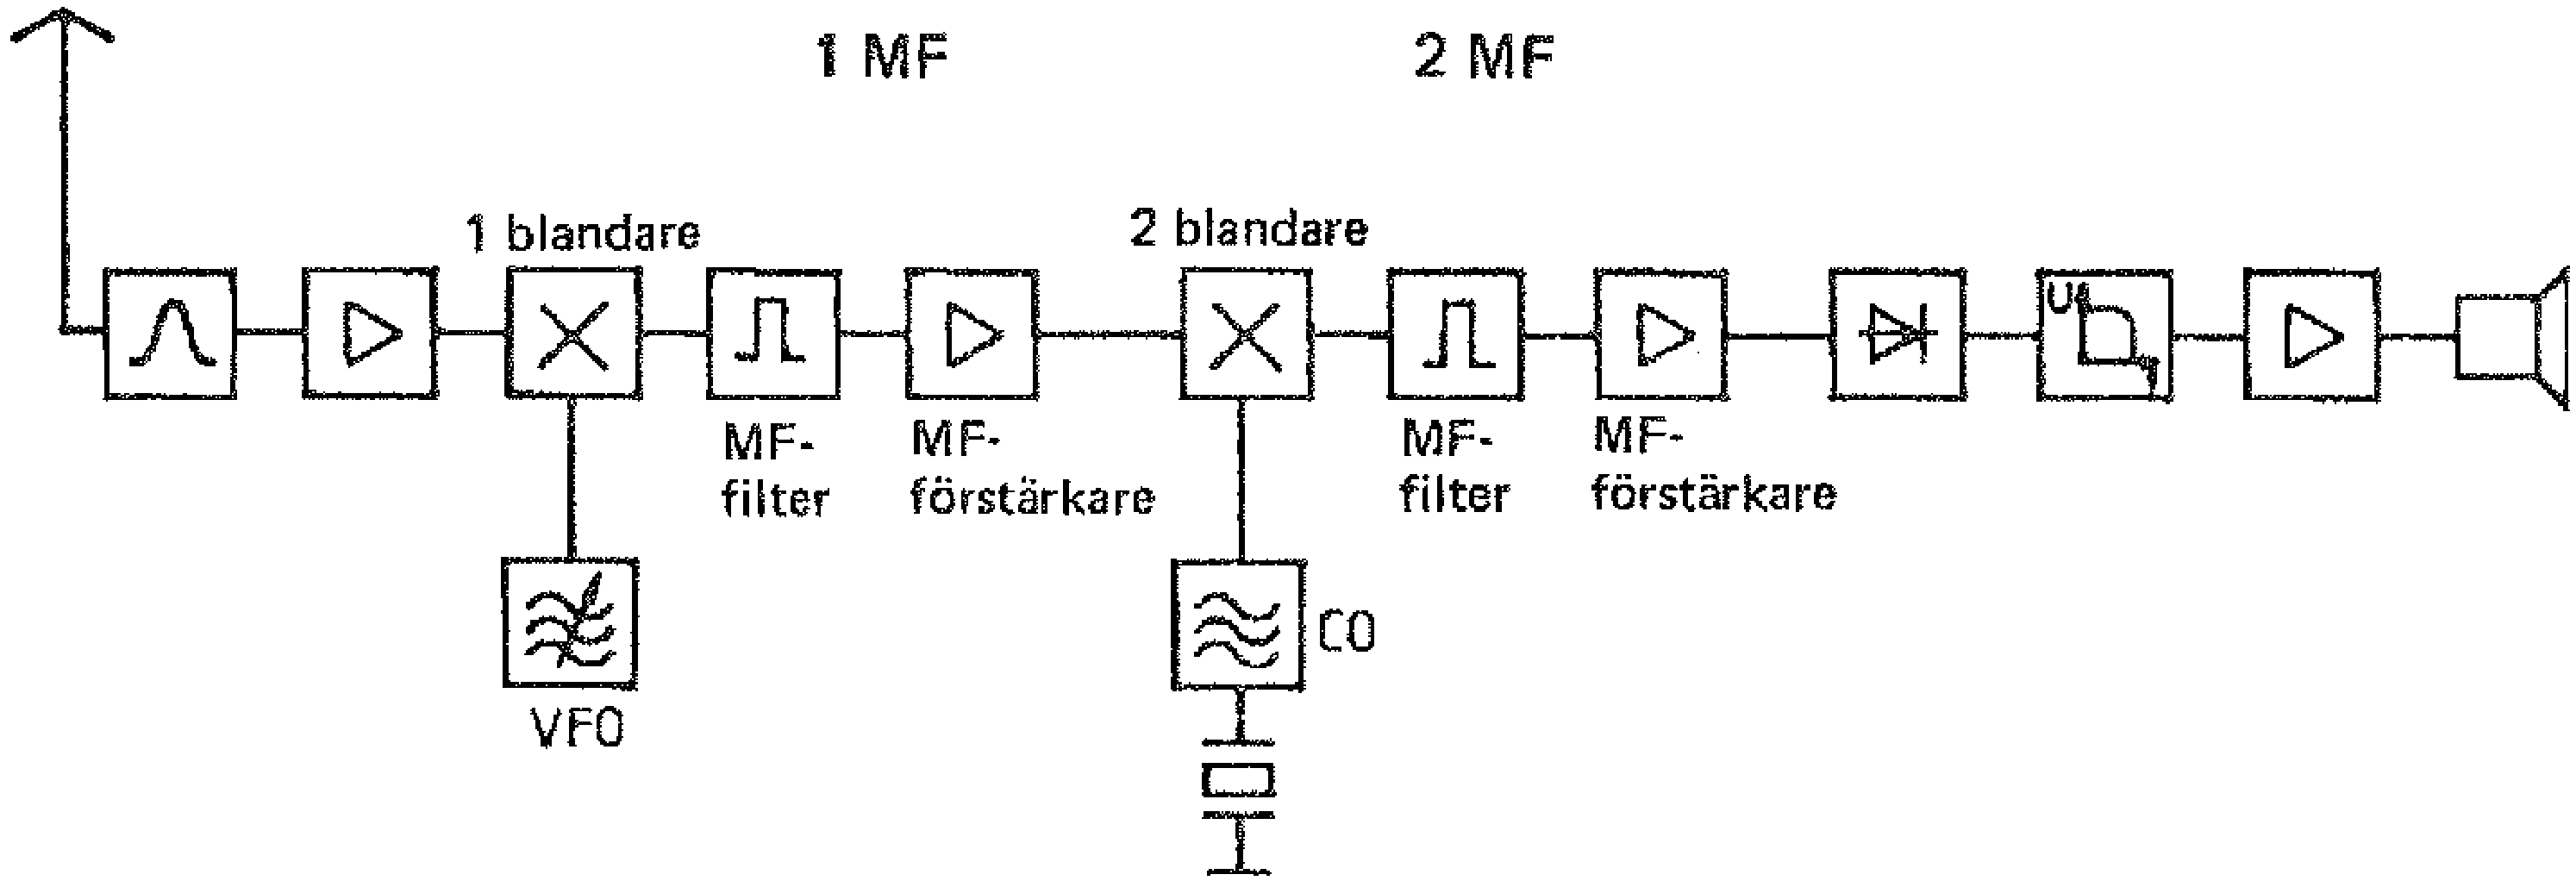
\includegraphics[width=\textwidth]{images/cropped_pdfs/bild_2_4-14.pdf}
  \caption{Dubbelsuperheteodynen i princip}
  \label{fig:bildII4-14}
\end{figure}

I ett MF-filter med centerfrekvensen 9~MHz skulle det behövas ett nära
20~gånger högre Q-värde för samma bandbredd 6~kHz

\[ Q = \frac{f_{res}}{b} = \frac{9000}{6} = 1500 \]

Ett så högt Q-värde kan endast erhållas med kristallfilter.

För högre mottagningsfrekvenser räcker det, på grund av filterproblematiken,
oftast inte med en dubbel frekvensomvandling.
Om man antar en dubbelsuper-mottagare för VHF-området 144--146~MHz enligt
bilden, så skulle en 1:a MF med frekvensen 10,7~MHz inte vara tillräckligt hög.
Vid en mottagningsfrekvens av 146~MHz är nämligen spegelfrekvensen
\(146 + (2 \cdot 10,7) = 167,4\)~MHz, alltså endast 1,15 gånger
mottagningsfrekvensen.
Det hade alltså varit lämpligt med en trippelsuper, det vill säga en trefaldig
frekvensomvandling, med en 1:a MF i frekvensområdet 70~MHz.
